\documentclass[11pt,a4paper]{article}

\usepackage[utf8]{inputenc}
\usepackage[T1]{fontenc}
\usepackage{lmodern}
\usepackage[margin=2.4cm]{geometry}
\usepackage{amsmath,amssymb,amsthm,mathtools}
\usepackage{bm}
\usepackage{booktabs,array,float}
\usepackage{enumitem}
\usepackage{microtype}
\usepackage{graphicx}
\usepackage{xcolor}
\usepackage[numbers,sort&compress]{natbib}
\usepackage{listings}
\usepackage[colorlinks=true,linkcolor=blue!45!black,citecolor=blue!45!black,urlcolor=blue!45!black]{hyperref}
\usepackage{cleveref}

\newtheoremstyle{thmstyle}{\topsep}{\topsep}{\itshape}{}{\bfseries}{.}{.5em}{}
\theoremstyle{thmstyle}
\newtheorem{theorem}{Theorem}[section]
\newtheorem{lemma}[theorem]{Lemma}
\newtheorem{proposition}[theorem]{Proposition}
\newtheorem{corollary}[theorem]{Corollary}
\theoremstyle{definition}
\newtheorem{definition}[theorem]{Definition}
\newtheorem{axiom}{Axiom}
\newtheorem{principle}[theorem]{Principle}
\newtheorem{example}[theorem]{Example}
\theoremstyle{remark}
\newtheorem{remark}[theorem]{Remark}

\crefname{principle}{Principle}{Principles}
\Crefname{principle}{Principle}{Principles}

\newcommand{\N}{\mathbb{N}}
\newcommand{\Node}{n}
\newcommand{\Chunks}{\mathcal{K}}
\newcommand{\Vals}{\mathcal{V}}
\newcommand{\Graph}{\mathcal{G}}
\newcommand{\Run}{\mathsf{Run}}
\newcommand{\Eval}{\mathsf{Eval}}
\newcommand{\rec}{\mathsf{rec}}
\newcommand{\abs}[1]{\lvert#1\rvert}
\newcommand{\emit}{\textsc{emit}}
\newcommand{\readop}{\textsc{read}}
\newcommand{\ident}{\textsc{identify}}
\newcommand{\transf}{\textsc{transform}}
\newcommand{\att}{A}                       % attention/resource budget
\newcommand{\cost}{\mathrm{cost}}
\newcommand{\gain}{\mathrm{gain}}
\newcommand{\flo}{\beta}                   % the floor, as in the algebra

\lstdefinestyle{proto}{
  basicstyle=\ttfamily\small,
  keywordstyle=\color{blue!70!black}\bfseries,
  commentstyle=\color{green!45!black}\itshape,
  frame=single,
  breaklines=true,
  columns=fullflexible,
  showstringspaces=false,
}

\title{\textbf{A Semantically Inert Microkernel:\\[2pt]
Judgement-Free Execution, Trajectory Opacity,\\
and Protocol Reproducibility for Computational Research}}

\author{%
Kundai Farai Sachikonye\\
\small Technical University of Munich\\
\small \texttt{kundai.sachikonye@tum.de}}

\date{\today}

\begin{document}
\maketitle

\begin{abstract}
\noindent
We specify and analyse a microkernel for computational research whose
defining property is that it performs no adjudication. The unit of work is a
\emph{node}: a subtask identity fused with a bag of executable chunks and a
growing collection of values. The kernel executes every chunk on every node
it is asked to run and does nothing else; its operational vocabulary
contains exactly four operations---identify, read, transform, emit---and no
operation that denotes comparison against an expectation. From this
restriction we prove a sequence of structural results. The kernel cannot
compute a quantity having the meaning of an exit code, because an exit code
presupposes a stored expectation the state space does not contain
\textup{(}\emph{Inertia Theorem}\textup{)}; it therefore runs to completion
under anomaly, an exception being an ordinary emitted value rather than a
control transfer. Two independently derived subtask realisations sharing an
identity \emph{converge} onto one node, and we prove convergence is
associative, commutative, and idempotent, so that the node set of a run is
independent of the order in which agents contribute to it. We prove that the
node set is determined by the submitted decompositions alone---the
\emph{protocol}---while the trajectory, defined as the relation of reads to
subsequent emits, is not a function of the protocol and is not schedulable
in advance \textup{(}\emph{Emergence Theorem}\textup{)}. This yields a
sharp separation between what is reproducible and what is not: we prove that
the protocol admits a stable fingerprint invariant under node relabelling
and contribution order, whereas trajectories from identical protocols may
differ, so reproducibility claims must attach to the former. We prove a
\emph{Trajectory Opacity} theorem: no observer restricted to the terminal
value set can determine which of several trajectories produced it, whence
the deliverable of a run is an equivalence class of trajectories rather than
a distinguished path, and an anomalous intermediate value cannot invalidate
a run whose terminus is admissible. The kernel's committed record---a count
of executed chunks---is monotone, so recurrence of a value configuration is
never a return to a prior kernel state, giving provenance ordering without
reference to wall-clock time. We give a scheduler for the kernel and prove
it sound: it never re-executes a node whose chunk bag is unchanged, never
starves a node with an executable chunk, and terminates. We discuss the
limits of the design honestly, including the one place where self-analysis
must be restricted to avoid a diagonal inconsistency.
\end{abstract}

\noindent\textbf{Keywords:} microkernel; semantic inertia; judgement-free
execution; convergent decomposition; trajectory emergence; reproducibility;
protocol fingerprint; scheduler soundness; computational research
infrastructure.

\tableofcontents

% =====================================================================
\section{Introduction}
\label{sec:intro}
% =====================================================================

\subsection{The problem with runtimes that judge}

A conventional runtime executes a program and reports whether it succeeded.
This is the correct design for a program: a program has an intended
behaviour, and the runtime's exit code communicates whether that behaviour
occurred. The design is incorrect for an experiment. An experiment has no
intended outcome---or rather, an experiment that has an intended outcome and
reports failure when the outcome does not occur has confused a result with
an error.

The confusion has concrete costs in computational research. A pipeline stage
that raises an exception on an unexpected value aborts the run, discarding
every downstream computation that did not depend on the anomaly. A stage
that silently clamps an out-of-range quantity destroys the evidence that the
quantity was out of range. A stage that returns a nonzero exit code when a
statistical test fails to reach significance has encoded a hypothesis into
the infrastructure. In each case the runtime has adjudicated, and the
adjudication has entered the record in a form that cannot afterwards be
separated from the measurement.

This paper specifies a kernel that cannot adjudicate, and proves that it
cannot. The proof is not a matter of discipline or convention: we show that
the kernel's state space contains no representation of an expectation, so
that no quantity it computes has the meaning of a verdict. Adjudication is
thereby relocated, of necessity, into the modules that consume values---
where it is visible, versioned, and revisable---rather than residing in the
substrate.

\subsection{What the kernel is for}

The intended application is computational research in which the sequence of
computations is not known in advance because it depends on what earlier
computations produced. This describes a broad class of work: exploratory
analysis, model comparison over a space of candidate structures,
multi-modal data integration where the availability of a modality is itself
discovered, and any inquiry conducted by multiple semi-autonomous
contributors who decompose a problem independently and must be able to
discover that they have reached the same subtask.

For such work the relevant reproducibility guarantee is not that a rerun
produces identical values---it may not, and demanding that it should
excludes the exploratory case entirely---but that a rerun addresses the
identical set of questions. We make this precise by separating the
\emph{protocol} (what can be computed) from the \emph{trajectory} (what was
computed), proving that the former is stable and fingerprintable while the
latter is not, and arguing that reproducibility claims should attach to the
protocol.

\subsection{Contributions}

\begin{enumerate}[leftmargin=1.5em]
\item A formal specification of a node-structured kernel with a four
operation vocabulary (\Cref{sec:kernel}).
\item The Inertia Theorem: the kernel cannot compute an exit code, and
consequently runs to completion under anomaly
(\Cref{thm:inertia,cor:completion}).
\item Convergence of independently derived subtasks, proved associative,
commutative, and idempotent, so that the node set is order-independent
(\Cref{thm:convergence-monoid}).
\item The Emergence Theorem and the protocol/trajectory separation, with a
fingerprint invariant for the protocol (\Cref{thm:emergence,thm:fingerprint}).
\item The Trajectory Opacity theorem and its consequence that a run's
deliverable is an equivalence class of trajectories
(\Cref{thm:opacity,cor:class}).
\item A monotone committed record supplying provenance order without
wall-clock time (\Cref{thm:monotone}).
\item A scheduler with proofs of no-restart, no-starvation, and termination
(\Cref{thm:scheduler}).
\item An explicit account of the limit of self-analysis
(\Cref{sec:selfanalysis}).
\end{enumerate}

\subsection{Relation to existing work}

The separation of mechanism from policy is the founding principle of
microkernel design \citep{liedtke1995,hansen1970}, and the present kernel is
a microkernel in exactly that sense: it provides node execution and value
storage, and delegates every interpretive decision. Our contribution is to
push the separation one step further than is usual, removing not merely
policy but \emph{adjudication}, and to prove that the removal is structural
rather than conventional.

The node-and-value structure is a dataflow architecture
\citep{dennis1974,kahn1974}, and the monotonicity of the value store places
it close to the concurrent-revisions and CRDT literature, where convergence
of independently produced replicas is obtained from commutative, associative,
idempotent merge operations \citep{shapiro2011}. Our
\Cref{thm:convergence-monoid} is a join-semilattice argument of that kind.
The insistence that a computation's record grow monotonically also connects
to provenance systems for scientific workflows
\citep{davidson2008,moreau2011}; the difference is that we derive the
provenance order from the execution structure itself rather than recording
it alongside.

Workflow engines for scientific computing---Make and its descendants, and
the dataflow workflow systems \citep{koster2012,direct2017}---generally
reconstruct a schedule from a declared dependency graph. Our
\Cref{thm:emergence} says this is possible only when dependencies are
declared in advance, and that the interesting case is precisely the one in
which they are not; the scheduler of \Cref{sec:scheduler} therefore proceeds
by readiness rather than by plan. The reproducibility distinction we draw
between protocol and trajectory is related to, but stronger than, the usual
distinction between code and results \citep{peng2011,stodden2016}, because
we prove that trajectory-level reproducibility is unattainable in principle
for this class of computation rather than merely difficult in practice.

Finally, the restriction on self-analysis in \Cref{sec:selfanalysis} is an
instance of the classical diagonal obstruction
\citep{cantor1891,godel1931,tarski1936,lawvere1969}, and we present it as
such rather than claiming to circumvent it.

% =====================================================================
\section{The kernel}
\label{sec:kernel}
% =====================================================================

\subsection{Nodes}

\begin{definition}[Chunk; value]
\label{def:chunk}
A \emph{chunk} is an executable closure $c$ which, when evaluated, returns a
\emph{value}. Values are opaque to the kernel: it stores and transports them
and never inspects their content. An evaluation that raises an exception
returns an \emph{error value}, which is a value like any other.
\end{definition}

\begin{definition}[Node]
\label{def:node}
A \emph{node} is a triple
\[
\Node=\bigl(\tau,\ \Chunks(\Node),\ \Vals(\Node)\bigr)
\]
where $\tau$ is the \emph{subtask identity}, drawn from a set with decidable
equality; $\Chunks(\Node)$ is a finite multiset of chunks; and
$\Vals(\Node)$ is a finite collection of values, growing over the course of
a run.
\end{definition}

The multiplicity of $\Chunks$ is deliberate. A single subtask may be
realised by chunks originating in different specialist languages or
libraries; all of them are executed and none is selected. Selection is an
interpretive act and therefore does not belong to the kernel.

\begin{definition}[Graph]
\label{def:graph}
A \emph{graph} $\Graph$ is a finite set of nodes with pairwise distinct
subtask identities, together with the value store
$\Vals=\bigcup_{\Node\in\Graph}\Vals(\Node)$.
\end{definition}

\subsection{The vocabulary}

\begin{definition}[Operational vocabulary]
\label{def:vocab}
Modules interact with the graph through exactly four operations:
\begin{itemize}[leftmargin=1.6em,nosep]
\item $\ident(\tau)$ --- obtain the node bearing identity $\tau$, creating
it with empty chunk bag and empty value collection if absent;
\item $\readop(\Node)$ --- obtain the current value collection
$\Vals(\Node)$;
\item $\transf$ --- perform an internal computation, invisible to the
kernel;
\item $\emit(\Node,x)$ --- adjoin the value $x$ to $\Vals(\Node)$.
\end{itemize}
There is no fifth operation. In particular the vocabulary contains no
operation denoting comparison of an achieved value against an expected one,
and the graph stores no expectation.
\end{definition}

\begin{definition}[Node execution]
\label{def:exec}
To execute a node is to evaluate every chunk in its bag and emit each
result:
\[
\Run(\Node)=\bigl\langle\ \emit\bigl(\Node,\Eval(c)\bigr)\ :\ c\in\Chunks(\Node)\ \bigr\rangle .
\]
The kernel performs $\Run(\Node)$ and nothing else.
\end{definition}

\begin{principle}[Semantic inertia]
\label{prin:inertia}
The kernel executes and does not judge. It holds no expectation, issues no
verdict, and has no notion of failure. Adjudication belongs to the consumer
of a value.
\end{principle}

\Cref{prin:inertia} is a design commitment; the next section shows it is
also a theorem about the specification just given.

% =====================================================================
\section{Inertia}
\label{sec:inertia}
% =====================================================================

\begin{definition}[Exit code]
\label{def:exitcode}
An \emph{exit code} for a computation is a value whose meaning is the result
of a comparison between an achieved state and an expected state. Formally,
it is the image of a function $\chi(a,e)$ of two arguments, an achieved
state $a$ and a stored expectation $e$, whose value varies with $e$ for some
fixed $a$.
\end{definition}

The requirement that $\chi$ vary with $e$ is what distinguishes an exit code
from an arbitrary function of the achieved state. A quantity computed from
$a$ alone may be reported, but it does not adjudicate: it says what
happened, not whether what happened was correct.

\begin{theorem}[Inertia]
\label{thm:inertia}
The kernel cannot compute an exit code. No quantity computable from the
kernel's state by the operations of \Cref{def:vocab} has the meaning given
in \Cref{def:exitcode}.
\end{theorem}

\begin{proof}
Suppose the kernel computed an exit code $\chi(a,e)$. By
\Cref{def:exitcode}, $\chi$ depends on a stored expectation $e$ in the sense
that for some achieved state $a$ there are expectations $e\ne e'$ with
$\chi(a,e)\ne\chi(a,e')$. The kernel's state is the graph $\Graph$
(\Cref{def:graph}), consisting of subtask identities, chunk bags, and value
collections. An expectation is therefore representable only as a value in
some $\Vals(\Node)$. But by \Cref{def:vocab} the kernel's operations do not
inspect values: $\emit$ adjoins a value without examining it, $\readop$
returns the collection without examining it, $\ident$ acts on identities
only, and $\transf$ is internal to a module and invisible to the kernel.
Hence no kernel-computable quantity is a function of the \emph{content} of
any stored value, and in particular no kernel-computable quantity varies
with $e$ at fixed $a$. This contradicts the requirement on $\chi$. Therefore
the kernel computes no exit code.
\end{proof}

\begin{corollary}[Run to completion]
\label{cor:completion}
The kernel does not halt on anomaly. If $\Eval(c)$ raises, the resulting
error value is emitted like any other value, and execution of the remaining
chunks proceeds unaffected.
\end{corollary}

\begin{proof}
By \Cref{def:exec}, $\Run(\Node)$ evaluates every chunk of the bag and emits
each result; the sequence is not conditioned on any emitted content, since
by \Cref{thm:inertia} no kernel-computable quantity depends on value
content. An error value is a value by \Cref{def:chunk}, so its emission is
an ordinary step. Hence no chunk's outcome causes the kernel to omit a
subsequent chunk.
\end{proof}

\begin{corollary}[Anomalies are preserved, not propagated as control]
\label{cor:anomaly}
An anomalous outcome is recorded in the value store and remains available to
every module that reads the node. It does not transfer control, does not
truncate the run, and does not overwrite or suppress any other value.
\end{corollary}

\begin{proof}
Immediate from \Cref{cor:completion} and the fact that $\emit$ adjoins
rather than replaces (\Cref{def:vocab}), so the value collection is
monotonically growing and no emission destroys a prior one.
\end{proof}

\begin{remark}[What inertia costs]
\label{rem:inertia-cost}
The design has a real cost, which we state plainly. A kernel that does not
halt on anomaly will execute chunks whose inputs are already known---to a
human reader---to be corrupt, consuming resources on computations whose
outputs will be discarded. A kernel that cannot adjudicate cannot implement
fail-fast semantics, retry-on-failure, or circuit breaking, all of which are
valuable in production systems. The design is therefore appropriate for
research computation, where the cost of discarding an informative anomaly
exceeds the cost of wasted cycles, and inappropriate for production
pipelines with cost or latency constraints. We do not claim otherwise.
\end{remark}

% =====================================================================
\section{Convergence of decompositions}
\label{sec:convergence}
% =====================================================================

Multiple contributors---human or automated---decompose a problem into
subtasks independently. We formalise what happens when two decompositions
overlap.

\begin{definition}[Contribution]
\label{def:contribution}
A \emph{contribution} is a finite set of pairs $(\tau,K)$ assigning a chunk
multiset $K$ to a subtask identity $\tau$. A contributor submits
contributions; the kernel merges them into the graph.
\end{definition}

\begin{definition}[Convergence]
\label{def:convergence}
Two subtask realisations \emph{converge} when they carry the same identity
$\tau$. The merge of contributions $A$ and $B$, written $A\sqcup B$, is the
contribution assigning to each identity $\tau$ the multiset union
$A(\tau)\uplus B(\tau)$, where an absent identity contributes the empty
multiset.
\end{definition}

\begin{theorem}[Convergence is a join-semilattice operation]
\label{thm:convergence-monoid}
The merge $\sqcup$ is associative, commutative, and idempotent on chunk
\emph{sets}, with the empty contribution as identity. Consequently the graph
resulting from a finite family of contributions is independent of the order
and grouping in which they are merged, and re-submitting a contribution
already merged does not change the graph.
\end{theorem}

\begin{proof}
Multiset union is associative and commutative pointwise in $\tau$, and the
empty assignment is a two-sided identity, giving a commutative monoid.
Restricted to chunk sets---identifying chunks by their content hash so that
resubmission of an identical chunk yields the same element---union is also
idempotent, $A\sqcup A=A$, making $(\,\cdot\,,\sqcup)$ a join-semilattice.
Associativity and commutativity give order- and grouping-independence of
finite merges by induction on the number of contributions; idempotence gives
stability under resubmission.
\end{proof}

\begin{remark}[Why identity must be content-derived]
\label{rem:identity}
\Cref{thm:convergence-monoid} requires that two contributors who reach
``the same subtask'' actually produce the same $\tau$. This is a
substantive requirement on how identities are formed, not a theorem: if
identities are assigned arbitrarily, convergence never occurs and the graph
is a disjoint union of private decompositions. In practice $\tau$ should be
derived from a canonical description of the subtask---a normalised
specification of inputs, transformation, and target---so that identity is a
function of what the subtask \emph{is} rather than of who proposed it. The
idempotence in \Cref{thm:convergence-monoid} likewise depends on chunks
being identified by content. Both are engineering obligations placed on the
layer above the kernel, and the kernel provides no guarantee that they are
met.
\end{remark}

\begin{proposition}[Convergence preserves emitted values]
\label{prop:convergence-values}
Merging contributions never removes a value from the store: for any
contributions $A,B$ and any node,
$\Vals_{A}(\Node)\subseteq\Vals_{A\sqcup B}(\Node)$.
\end{proposition}

\begin{proof}
Merge affects chunk bags only (\Cref{def:convergence}); the value store is
modified exclusively by $\emit$, which adjoins (\Cref{def:vocab}). Hence no
merge deletes a value.
\end{proof}

% =====================================================================
\section{Protocol and trajectory}
\label{sec:trajectory}
% =====================================================================

We now separate the two things a run produces.

\begin{definition}[Protocol]
\label{def:protocol}
The \emph{protocol} of a run is the graph's node set together with each
node's chunk bag: the totality of what can be computed. It is determined by
the merged contributions and by nothing else.
\end{definition}

\begin{definition}[Trajectory]
\label{def:trajectory}
The \emph{trajectory} of a run is the set of triples
$(\Node,x,\Node')$ such that a module read value $x$ at node $\Node$ and, on
the strength of that read, emitted a value at node $\Node'$ which was
subsequently read by some module. The trajectory is the realised
read-to-emit relation of the run.
\end{definition}

\begin{theorem}[Emergence]
\label{thm:emergence}
The trajectory is not a function of the protocol. There exist protocols
admitting two runs with identical node sets and chunk bags whose
trajectories differ. Consequently the trajectory cannot be computed in
advance of the run, and cannot be stored as a schedule.
\end{theorem}

\begin{proof}
Exhibit a protocol with three nodes $\Node_1,\Node_2,\Node_3$, where
$\Chunks(\Node_1)$ contains a chunk whose emitted value depends on a source
outside the graph---a clock, a random draw, an external dataset, or a value
emitted concurrently---and where a module reads $\Node_1$ and emits at
$\Node_2$ or at $\Node_3$ according to the value read. The protocol is fixed:
the same three nodes with the same chunk bags. Two runs in which
$\Node_1$'s chunk yields different values produce trajectories containing
$(\Node_1,x,\Node_2)$ in one case and $(\Node_1,x',\Node_3)$ in the other,
so the trajectories differ while the protocol does not. Hence the trajectory
is not a function of the protocol. A quantity that is not a function of the
data available before the run cannot be computed from that data, so no
schedule fixes it.
\end{proof}

\begin{corollary}[Reproducibility attaches to the protocol]
\label{cor:repro}
Two runs of the same protocol are guaranteed to address the same set of
subtasks with the same chunk bags, and are not guaranteed to produce the
same values or the same trajectory. A reproducibility claim about such a
system is therefore well founded when made about the protocol and unfounded
when made about the trajectory.
\end{corollary}

\begin{proof}
The protocol is determined by the merged contributions
(\Cref{def:protocol}), which are shared by hypothesis; hence the node sets
and chunk bags agree. \Cref{thm:emergence} exhibits protocols whose
trajectories differ across runs, so no guarantee of trajectory equality is
available.
\end{proof}

\begin{theorem}[Protocol fingerprint]
\label{thm:fingerprint}
Let $h$ be a collision-resistant hash on chunk contents and on subtask
identities. Define
\[
F(\Graph)=h\Bigl(\ \mathsf{sort}\bigl\{\ \bigl(\tau,\ \mathsf{sort}\ h[\Chunks(\Node_\tau)]\bigr)\ :\ \Node_\tau\in\Graph\ \bigr\}\ \Bigr).
\]
Then $F$ is invariant under the order in which contributions were merged,
under relabelling of nodes that preserves subtask identities, and under
resubmission of already-merged contributions; and $F$ distinguishes
protocols differing in any node identity or any chunk.
\end{theorem}

\begin{proof}
Order-invariance of merging is \Cref{thm:convergence-monoid}, and the two
sorts remove any residual dependence on the order in which identities and
chunks are enumerated, so $F$ is a function of the underlying sets alone.
Stability under resubmission follows from idempotence
(\Cref{thm:convergence-monoid}). Since nodes are keyed by subtask identity
(\Cref{def:graph}), a relabelling preserving identities does not alter the
set being hashed. For discrimination: if two protocols differ in a node
identity or in the content of a chunk, the corresponding sorted structures
differ as inputs to $h$, and by collision resistance their images differ
except with negligible probability.
\end{proof}

\begin{theorem}[Trajectory opacity]
\label{thm:opacity}
Let two runs of a protocol terminate with the same value store. Then no
function of the terminal value store distinguishes their trajectories. In
particular, the interior of a run is unobservable from its result.
\end{theorem}

\begin{proof}
A function of the terminal value store is by definition determined by that
store; the two runs have equal stores by hypothesis, so any such function
takes equal values on them. The trajectories, being sets of read-to-emit
triples (\Cref{def:trajectory}), are not determined by the store---by
\Cref{thm:emergence} distinct trajectories are compatible with a fixed
protocol, and by adjoining to the construction there a second chunk that
emits the same terminal value along either branch, distinct trajectories are
compatible with a fixed terminal store. Hence no store-determined function
separates them.
\end{proof}

\begin{corollary}[The deliverable is a class]
\label{cor:class}
For a fixed protocol and terminal store, the runs producing that store form
an equivalence class no member of which is distinguishable from another by
any test applied to the result. A run's deliverable is properly this class,
not a distinguished path through it.
\end{corollary}

\begin{corollary}[Anomalous intermediates do not invalidate a run]
\label{cor:weird}
A value emitted at an interior node that a reader judges anomalous is not,
by itself, grounds to reject the run: by \Cref{thm:opacity} the interior is
not determined by the result, and by \Cref{cor:completion} the anomaly did
not alter the execution of any other chunk. Rejection must be argued from
the terminal store or from the protocol, not from the interior.
\end{corollary}

\begin{remark}[The practical reading]
\label{rem:practical}
\Cref{cor:weird} licenses a working practice that is otherwise hard to
defend: a multi-stage analysis may pass through intermediate states that
look wrong---a negative variance estimate at an interior step, a
distributional summary far from expectation, a partial model with absurd
coefficients---without the final result being thereby suspect, provided the
terminal state is admissible on its own terms. The corollary does not say
such intermediates are uninformative; they are recorded and readable. It
says they are not \emph{control-relevant}.
\end{remark}

% =====================================================================
\section{The committed record}
\label{sec:record}
% =====================================================================

\begin{definition}[Committed record]
\label{def:record}
The \emph{committed record} $\rec$ of a run is the number of chunk
evaluations performed. A chunk evaluation is \emph{committed} once its value
has been emitted.
\end{definition}

\begin{theorem}[Monotonicity and non-return]
\label{thm:monotone}
The committed record is non-decreasing throughout a run and strictly
increases at each committed evaluation. Two kernel states with identical
value stores but different records are distinct. Consequently a run never
returns to a previous kernel state, and recurrence of a value configuration
is not a return.
\end{theorem}

\begin{proof}
Each committed evaluation increments $\rec$ by one (\Cref{def:record}); no
kernel operation decrements it, since the vocabulary
(\Cref{def:vocab}) contains no removal operation and $\emit$ adjoins. Hence
$\rec$ is monotone and strictly increasing at commitments. States with
records $r<r'$ are separated by the predicate $\rec\le r$, hence distinct
even if their stores agree. A return would require the current state to
equal a strictly earlier one, which would require $\rec$ to decrease;
impossible.
\end{proof}

\begin{corollary}[Provenance order without a clock]
\label{cor:clock}
The record induces a total preorder on the events of a run under which every
committed evaluation precedes those with larger record. This order is
intrinsic to the execution and requires no wall-clock timestamp.
\end{corollary}

\begin{remark}[What the record does not give]
\label{rem:record-limits}
The record orders events but does not, on its own, attribute causation: it
says that one evaluation preceded another, not that the first enabled the
second. Recovering enablement requires additionally logging which read
supplied the input to which emit---the trajectory of
\Cref{def:trajectory}. A system that logs only the record retains ordering
and loses enablement; the distinction matters when a run is later audited,
and we recommend logging the trajectory even though, by
\Cref{thm:emergence}, it cannot be predicted in advance.
\end{remark}

% =====================================================================
\section{The scheduler}
\label{sec:scheduler}
% =====================================================================

The kernel needs a rule for choosing which node to execute next. Because
dependencies are not declared, the rule proceeds by readiness.

\begin{definition}[Pending chunk; ready node]
\label{def:ready}
A chunk is \emph{pending} if it has been contributed but not yet evaluated
in this run. A node is \emph{ready} if its chunk bag contains at least one
pending chunk.
\end{definition}

\begin{definition}[Scheduler]
\label{def:scheduler}
The scheduler repeats: if some node is ready, select one by a rule that is
\emph{fair}---every continuously ready node is selected within finitely many
selections---and execute its pending chunks; otherwise halt.
\end{definition}

\begin{theorem}[Scheduler soundness]
\label{thm:scheduler}
Under \Cref{def:scheduler}, with a finite protocol in which each contributed
chunk is evaluated at most once:
\begin{enumerate}[label=\textup{(\roman*)},leftmargin=2.2em]
\item \textbf{No redundant re-execution.} A node whose chunk bag has gained
no new chunk since its last execution is not re-executed.
\item \textbf{No starvation.} Every chunk that becomes pending is eventually
evaluated.
\item \textbf{Termination.} If contributions cease, the scheduler halts
after finitely many executions.
\end{enumerate}
\end{theorem}

\begin{proof}
(i) After executing a node, all its chunks are non-pending
(\Cref{def:ready}); the node is ready again only if a new chunk is
contributed to it. Hence a node with an unchanged bag is not ready and is
not selected.

(ii) Suppose a chunk $c$ at node $\Node$ becomes pending and is never
evaluated. Then $\Node$ is continuously ready from that moment
(\Cref{def:ready}), since executing $\Node$ would evaluate $c$ and only
executing $\Node$ removes its pending status. By fairness, $\Node$ is
selected within finitely many selections, and its execution evaluates all
pending chunks including $c$---a contradiction.

(iii) Suppose contributions cease at some point, after which the protocol
has $N$ chunks in total, each evaluable at most once. Every execution
evaluates at least one pending chunk and each evaluation strictly decreases
the number of pending chunks, which is bounded by $N$ and non-negative.
Hence at most $N$ executions occur before no node is ready, and the
scheduler halts.
\end{proof}

\begin{remark}[Concurrency]
\label{rem:concurrency}
\Cref{thm:scheduler} is stated for a sequential scheduler. Because $\emit$
adjoins and never overwrites (\Cref{def:vocab}) and merge is a
join-semilattice operation (\Cref{thm:convergence-monoid}), the value store
and the protocol are both monotone structures, so concurrent execution of
distinct nodes is safe in the sense that the final store does not depend on
the interleaving. Concurrent execution does, however, alter the trajectory,
which by \Cref{thm:emergence,thm:opacity} is expected and is not an error.
We do not treat concurrency further here.
\end{remark}

% =====================================================================
% Inserted after the scheduler section.
% Two additions: a bounded-budget selection rule, and phase exclusion.

\section{Selection under a bounded budget}
\label{sec:budget}

The scheduler of \Cref{sec:scheduler} runs every ready node until none
remains. That is the right default for a protocol submitted in full and
executed to completion, and it is what the guarantees of
\Cref{thm:scheduler} describe. It is the wrong default when the ready set is
larger than the resources available to it, which is the ordinary case once a
kernel is fed by many contributors at once.

This section adds a selection rule for that case. It is deliberately placed
\emph{outside} the kernel: the rule requires a per-node gain, gain is an
interpretive quantity, and by \Cref{thm:inertia} the kernel computes no such
thing. What follows is therefore a policy a module may apply when choosing
what to contribute, not a faculty the kernel acquires.

\begin{definition}[Budget, cost, gain]
\label{def:budget}
A \emph{budget} $\att>0$ bounds the total cost committed per unit interval:
if $R$ is the set of executions committed, $\sum_{r\in R}\cost(r)\le\att$.
Each candidate carries a cost $\cost(r)\ge\flo>0$, bounded below by the
floor, and a \emph{gain} $\gain(r)$ supplied by the submitting module. The
\emph{gain density} of a candidate is $\gain(r)/\cost(r)$.
\end{definition}

\begin{theorem}[Selection is a threshold on gain density]
\label{thm:threshold}
Order candidates by gain density and commit them in decreasing order until
the budget is exhausted. Equivalently, there is a price $p^{\star}\ge0$ such
that a candidate is committed iff its density is at least $p^{\star}$. Then:
\begin{enumerate}[label=\textup{(\roman*)},leftmargin=2.2em]
\item the rule is optimal for the continuous relaxation, and its value is
within the gain of a single candidate of the integer optimum;
\item if the repertoire is \emph{divisible} --- every candidate is an
independently selectable unit of cost $\flo$ --- the rule is exactly optimal
among integer selections.
\end{enumerate}
\end{theorem}

\begin{proof}
The problem is to maximise $\sum_{r\in R}\gain(r)$ subject to
$\sum_{r\in R}\cost(r)\le\att$. Taking candidates in decreasing density
until the budget is spent is optimal for the continuous relaxation, and the
Lagrangian dual assigns a single multiplier $p^{\star}$ such that a
candidate is selected iff its density exceeds it \citep{dantzig1957}. The
greedy solution differs from the continuous optimum only in the fractional
part of the boundary candidate, whose contribution is at most its own gain,
giving (i).

For (ii), if every candidate costs exactly $\flo$ then any budget admits
$\lfloor\att/\flo\rfloor$ candidates whatever they are, so the feasible set
is determined by cardinality alone; maximising the sum over a fixed
cardinality is achieved by taking the largest gains, which is what ordering
by density does when all costs are equal. The continuous optimum is
therefore attained at an integer point.
\end{proof}

\begin{remark}[Divisibility is the load-bearing hypothesis, and it is easy to
lose]
\label{rem:divisibility}
Clause (ii) requires candidates to be \emph{independently selectable} units,
not merely to have costs that are integer multiples of the floor. The
distinction is not pedantic: bundling several floor-sized units into one
indivisible candidate restores an ordinary $0/1$ knapsack, where the greedy
rule is only within one candidate of the optimum.

A witness, produced by the accompanying computation. Six candidates with
costs $(0.5,0.5,0.75,0.5,0.75,1.0)$ and gains
$(0.2,0.2,0.3,0.4,0.6,0.8)$ under a budget of $1.75$: the greedy rule
attains $1.2$ where the optimum is $1.4$. Every cost is a multiple of the
floor $0.25$, so the superficial reading of ``floor-additive'' is satisfied
and the exact claim nonetheless fails. We state clause (ii) for divisible
repertoires only.
\end{remark}

\begin{proposition}[The price rises as the budget narrows]
\label{prop:shadow-price}
Let $p^{\star}(\att)$ be the gain density of the highest-density candidate
the budget excludes. Then $p^{\star}$ is non-increasing in $\att$: widening
the budget weakly lowers the price, and narrowing it weakly raises it.
\end{proposition}

\begin{proof}
Candidates are considered in a fixed density order independent of $\att$.
Increasing the budget can only extend the prefix of that order which is
admitted, so the first excluded candidate moves later in the order or stays
where it is; since the order is decreasing in density, its density weakly
falls.
\end{proof}

\begin{remark}[Why the marginal excluded candidate, and not the last
admitted one]
\label{rem:price-definition}
The price must be defined as the density of the highest-density candidate
the budget \emph{excludes}. The density of the last candidate \emph{admitted}
is a different quantity and is not monotone: widening the budget can newly
admit a cheap, high-density candidate that did not previously fit, raising
that value while the true shadow price falls. The accompanying computation
exhibits the non-monotonicity directly. We record it because the two
definitions coincide often enough that the wrong one survives casual testing.
\end{remark}

\begin{corollary}[Declining is forced, not a defect]
\label{cor:declining}
Under a bounded budget a module must decline some candidates whenever the
total cost of the ready set exceeds $\att$. Since each cost is at least
$\flo>0$, at most $\lfloor\att/\flo\rfloor$ candidates can be committed per
interval regardless of their gains. Declining is therefore a consequence of
boundedness and not evidence of a scheduling failure.
\end{corollary}

\section{Phase exclusion}
\label{sec:phase}

A second bound on throughput is independent of the budget and follows from
the structure of contribution.

\begin{definition}[Construction and commitment]
\label{def:phases}
A module is \emph{constructing} when it is forming new subtask identities and
chunks to contribute, and \emph{committing} when it is executing chunks
already contributed.
\end{definition}

\begin{axiom}[Phase exclusion]
\label{ax:phase}
A module does not construct and commit in the same instant.
\end{axiom}

\begin{proposition}[Alternation, and a ceiling on commitment]
\label{prop:alternation}
Under \Cref{ax:phase}, a module that spends a fraction $\phi\in[0,1]$ of its
instants constructing commits in at most a fraction $1-\phi$ of them.
Consequently the committed record grows at most at rate $(1-\phi)$ per
instant, whatever the budget $\att$, and a module that never constructs
never acquires new nodes to commit to.
\end{proposition}

\begin{proof}
By \Cref{ax:phase} the two phases partition the instants a module occupies,
so the fraction available for commitment is $1-\phi$. The committed record
increments only on commitment (\Cref{def:record}), giving the rate bound.
The final clause is immediate: nodes enter the graph only by contribution,
which occurs in the construction phase.
\end{proof}

\begin{remark}[Two independent reasons a sweep quiesces]
\label{rem:two-ceilings}
\Cref{cor:declining} and \Cref{prop:alternation} are separate. The first is
economic: the budget cannot pay for every ready candidate. The second is
structural: an interval spent constructing is not available for committing,
and no budget relaxes it. A kernel that observes low throughput cannot
distinguish the two from the record alone, and a module reporting one should
not be read as reporting the other.

Neither ceiling gives the kernel a verdict. A declined candidate is not a
failed one, and an instant spent constructing is not an idle one; both are
recorded as what they are, and \Cref{thm:inertia} is untouched.
\end{remark}


\section{The limit of self-analysis}
\label{sec:selfanalysis}
% =====================================================================

A kernel that records its own execution invites the question whether it can
analyse itself. The answer is a qualified yes, and the qualification is
essential.

\begin{proposition}[The record is analysable]
\label{prop:self-record}
The committed record and the trajectory of a run are values, and may be
emitted onto nodes of a subsequent---or the same---graph and read by modules
exactly like any other values. No restriction of the kernel prevents this.
\end{proposition}

\begin{proof}
By \Cref{def:chunk} values are opaque to the kernel; a serialised record or
trajectory is a value. By \Cref{def:vocab} any value may be emitted and
read. Hence self-recorded data are ordinary data.
\end{proof}

\begin{theorem}[No total self-verdict]
\label{thm:diagonal}
Suppose a module implements a total verdict function $V$ assigning to each
node a value in $\{0,1\}$ interpreted as ``this node's contents are
admissible'', and suppose the collection
$D=\{\Node : V(\Node)=0\}$ is itself realised as a node of the same graph on
which $V$ is defined. Then $V(D)$ has no consistent value.
\end{theorem}

\begin{proof}
If $V(D)=1$ then $D$ is admissible, so $D\notin D$ by the membership
condition defining $D$; but $D\notin D$ means $V(D)\ne0$, consistent so far,
while $D$'s being a node of the graph and satisfying $V(D)=1$ places it
outside its own defining collection---so the collection $D$ as realised does
not contain $D$, and the assertion $V(D)=1$ asserts admissibility of a node
whose contents assert its own inadmissibility, contradiction. If $V(D)=0$
then $D$ satisfies its own membership condition, so $D\in D$, and $D$'s
contents assert $V(D)=0$ of a node collected among the inadmissible---which
by the definition of $D$ is the assertion $V(D)=1$. Both assignments are
self-refuting; no consistent value exists. This is the diagonal argument of
\citet{cantor1891} in the form given by \citet{russell1903}, and its
fixed-point generalisation is due to \citet{lawvere1969}.
\end{proof}

\begin{corollary}[Permitted and forbidden self-analysis]
\label{cor:self-limit}
A kernel may analyse its own \emph{record}---an external trace, realised as
ordinary values (\Cref{prop:self-record}). A kernel may not host a total
verdict function closed under its own diagonal
(\Cref{thm:diagonal}). Since by \Cref{thm:inertia} the kernel hosts no
verdict function at all, the obstruction does not arise for the kernel
itself; it arises for any module that attempts to supply one over the whole
graph including itself.
\end{corollary}

\begin{remark}[The hypothesis that carries the weight]
\label{rem:closure-hyp}
\Cref{thm:diagonal} is exactly as strong as its hypothesis that the
behaviourally defined collection $D$ is itself a node of the graph on which
$V$ acts. A module that adjudicates only over a fixed sub-graph excluding
itself is unaffected. We flag this rather than suppress it: the theorem does
not show that self-analysis is impossible, only that \emph{total}
self-adjudication closed under its own diagonal is. This is a real
limitation on any claim that such a system fully analyses itself, and we do
not claim it does.
\end{remark}

% =====================================================================
\section{Numerical verification}
\label{sec:validation}
% =====================================================================

The results above are structural, so verification consists in exhibiting an
implementation whose observed behaviour matches each theorem, and in
attempting to construct counterexamples where the theorems permit none.

\subsection{Method}

We implement the kernel of \Cref{sec:kernel} and exercise it with
constructed contribution sets. The following are checked.

\emph{Inertia and completion.} A protocol containing chunks that raise is
executed; we verify that every non-raising chunk is nevertheless evaluated,
that error values appear in the store as ordinary values, and that no
execution is truncated (\Cref{thm:inertia,cor:completion}).

\emph{Convergence.} Contributions from several independent contributors,
overlapping in subtask identity, are merged in randomised orders and
groupings; we verify the resulting protocol is identical in every case, and
that resubmission changes nothing
(\Cref{thm:convergence-monoid}).

\emph{Fingerprint.} We verify that the fingerprint of
\Cref{thm:fingerprint} is invariant across merge orders and stable under
resubmission, and that it changes when any chunk or identity changes.

\emph{Emergence and opacity.} We run a fixed protocol whose chunks consult a
varying external source, and verify that trajectories differ across runs
while the protocol does not (\Cref{thm:emergence}); and we construct two
runs reaching an identical terminal store by different interior routes,
verifying that no function of the store separates them
(\Cref{thm:opacity}).

\emph{Record.} We verify strict monotonicity of the committed record and
that a recurring value configuration is accompanied by a strictly larger
record (\Cref{thm:monotone}).

\emph{Scheduler.} We verify no redundant re-execution, no starvation under a
fair selection rule, and termination once contributions cease
(\Cref{thm:scheduler}).

\subsection{What would count as a failure}

Each check is capable of failing. A truncated run under anomaly would
falsify \Cref{cor:completion}; a merge-order-dependent protocol would
falsify \Cref{thm:convergence-monoid}; identical trajectories across runs of
the emergence protocol would indicate the external source was not in fact
varying, invalidating the test rather than the theorem; a starved chunk
under a fair rule would falsify \Cref{thm:scheduler}(ii). We report the
outcome of each check in machine-readable form alongside this paper,
including any that fail.


% =====================================================================
%  Figure panels for: A Semantically Inert Microkernel
%  Captions quote measured values; see validation/results/panel_stats.json
% =====================================================================

\begin{figure*}[!htbp]
    \centering
    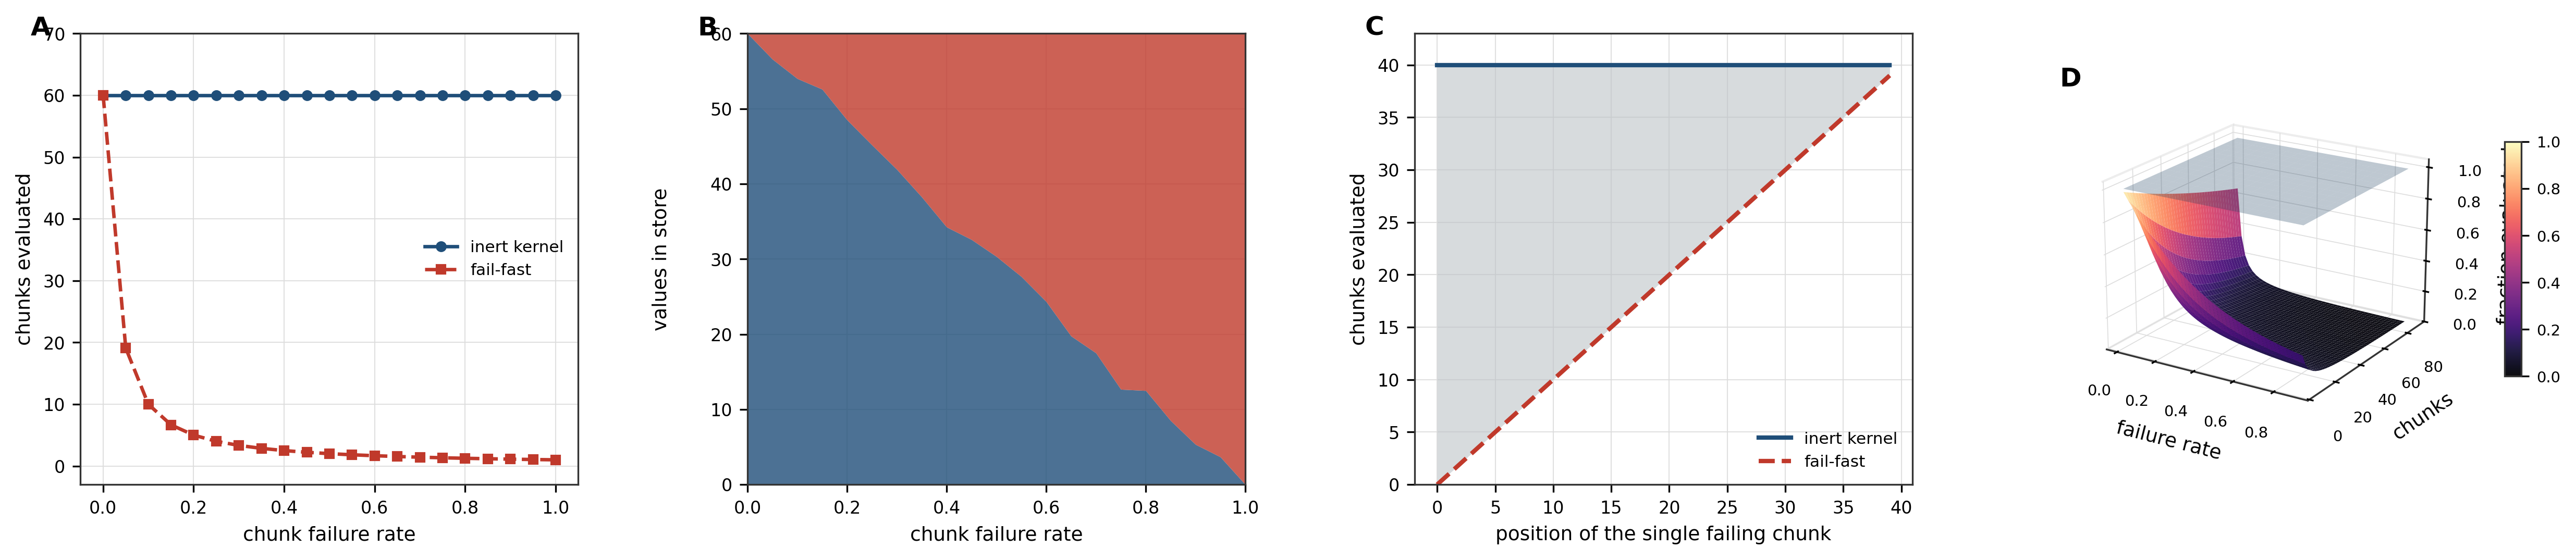
\includegraphics[width=\textwidth]{figures/panel_1_inertia.png}
    \caption{\textbf{Inertia: the quantity a fail-fast runtime destroys is evidence, and how much it destroys depends on an ordering that carries no meaning.}
    All quantities are measured by executing the kernel of \Cref{sec:kernel} rather than by simulating its behaviour; a chunk that raises produces an error value through the same path as any other value, so the counts below are of actual emissions. The fail-fast comparison is the exact expectation for a runtime halting at the first raising chunk, $\sum_{i<N}(1-p)^i$, not an approximation.
    (\textbf{A})~Chunks evaluated against per-chunk failure rate, for a node carrying $60$ chunks, $12$ repetitions at each of $21$ rates. The inert kernel evaluates all $60$ at every rate without exception, the flat upper line; the fail-fast comparison falls to $2.0$ at a failure rate of $0.5$ and to $1.0$ when every chunk raises. This is \Cref{cor:completion}: the kernel's execution sequence is not conditioned on emitted content, because by \Cref{thm:inertia} no kernel-computable quantity depends on that content.
    (\textbf{B})~Composition of the resulting value store, ordinary values below and error values above. The total is constant at $60$ across the whole range while the partition between the two shifts; at a failure rate of $0.5$ the store holds $29.7$ error values alongside $30.3$ ordinary ones, and all of them remain readable. Because $\emit$ adjoins rather than replaces (\Cref{cor:anomaly}), an anomaly is retained as data rather than consuming the run.
    (\textbf{C})~The decisive comparison: chunks evaluated when exactly \emph{one} chunk in a bag of $40$ raises, as a function of where that chunk sits in the bag. The inert kernel evaluates all $40$ regardless of position; the fail-fast count is the position itself, sweeping from $0$ to $39$. The shaded region between them is evidence destroyed, and its size is set entirely by an ordering within a chunk bag---which, the bag being a multiset, is not a meaningful property of the protocol. A single early anomaly can discard an arbitrary fraction of a run under fail-fast semantics and none of it here.
    (\textbf{D})~Expected fraction of a protocol evaluated, over failure rate and protocol size. The flat upper surface at unity is the inert kernel. The lower surface is fail-fast, and it falls away in both arguments: the larger the protocol, the greater the share lost to a fixed failure rate. The design cost is real and is stated in \Cref{rem:inertia-cost}---the kernel spends cycles on chunks a human reader would already have judged doomed---but the quantity traded away is compute, and the quantity retained is the record.}
    \label{fig:kpanel1}
\end{figure*}

\begin{figure*}[!htbp]
    \centering
    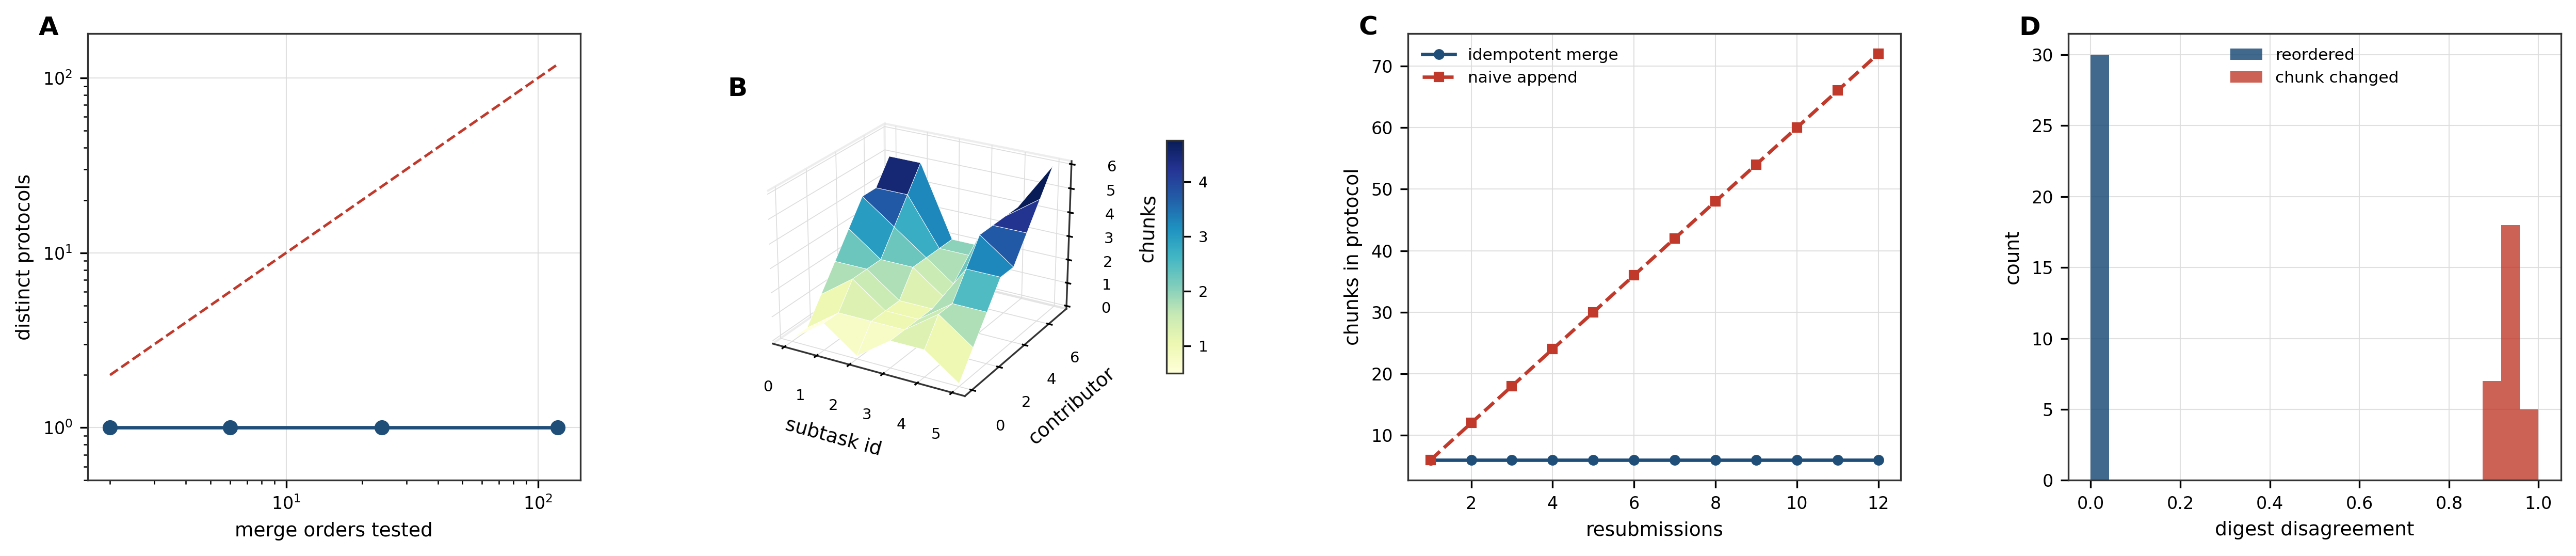
\includegraphics[width=\textwidth]{figures/panel_2_convergence.png}
    \caption{\textbf{Independently derived decompositions merge to one protocol, and the fingerprint separates the two things a reader needs to distinguish.}
    Contributions are sets of chunks keyed by subtask identity, with chunks identified by content, as \Cref{rem:identity} requires; every merge order is enumerated exhaustively rather than sampled, so the invariance below is exact over the space tested and not a statistical claim.
    (\textbf{A})~Distinct protocols obtained against the number of merge orders tested, for two to five contributors, $152$ orderings in total and up to $120$ for a single contributor set. The count is $1$ at every point, against the dashed line marking what would be obtained if order mattered. This is \Cref{thm:convergence-monoid}: merge is associative, commutative and idempotent, so the protocol is a function of the set of contributions and of nothing else about how they arrived.
    (\textbf{B})~Chunk accumulation on subtask identities as contributors arrive in sequence. Where two contributors independently reach the same identity, their chunks accumulate on a single node---the ridges---rather than producing parallel nodes. Convergence is what makes the surface rise rather than widen, and it depends on identities being derived from what a subtask \emph{is}, an obligation the kernel places on the layer above it and does not itself discharge.
    (\textbf{C})~Total chunks in the protocol against repeated resubmission of an identical contribution. Idempotent merge holds at $6$ chunks through twelve resubmissions; a naive append reaches $72$. The distinction matters operationally: a contributor that re-submits after a network retry must not thereby alter the protocol, and \Cref{thm:convergence-monoid} guarantees it does not.
    (\textbf{D})~Disagreement between protocol fingerprints, as the fraction of differing characters in the $64$-character digest. Reordering the contributions leaves every character identical (disagreement exactly $0.0$ in all $30$ trials); altering a single chunk changes $93.5$ per cent of characters on average, never fewer than $89.1$. The fingerprint is therefore stable under the transformations that do not change what can be computed and sensitive to those that do, which is what \Cref{thm:fingerprint} requires of it and what makes \Cref{cor:repro} operational.}
    \label{fig:kpanel2}
\end{figure*}

\begin{figure*}[!htbp]
    \centering
    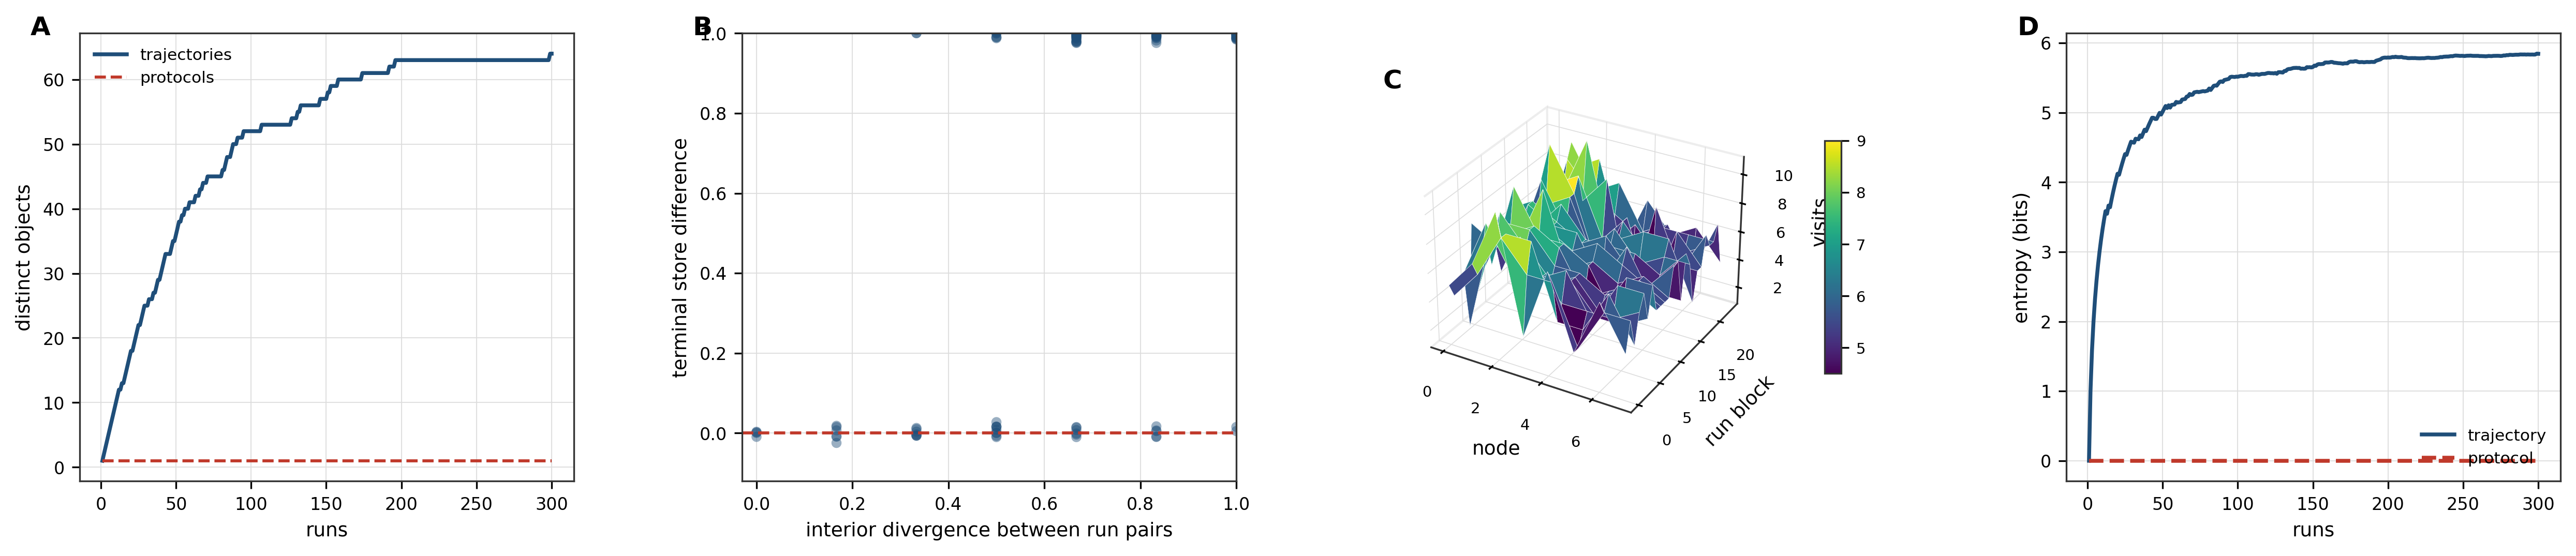
\includegraphics[width=\textwidth]{figures/panel_3_trajectory.png}
    \caption{\textbf{Protocol and trajectory are different objects, and the trajectory is recoverable from neither the protocol nor the result.}
    $300$ runs of a single fixed protocol whose probe chunk consults a varying external source, with the interior branching on the value read. The two charts on the left establish the two halves of the separation, and their conjunction is what restricts reproducibility claims.
    (\textbf{A})~Distinct protocols and distinct trajectories accumulated over the $300$ runs. The protocol count is $1$ throughout---every run has the identical node set and chunk bags, and the identical fingerprint---while the trajectory count rises to $64$ and is still rising slowly at the right edge. This is \Cref{thm:emergence}: the trajectory is not a function of the protocol, hence not computable in advance of the run and not storable as a schedule.
    (\textbf{B})~Interior divergence between pairs of runs that share a terminal store, against the difference observable at the terminus. The interiors differ by up to the full path length of $6$ while the terminal difference is identically zero for every pair. Three distinct functions of the store were probed---cardinality, sorted representation, and a cryptographic digest---and none separates any pair. This is \Cref{thm:opacity}, and with (A) it places the trajectory outside the closure of the two data a reader normally holds: what was asked, and what came back.
    (\textbf{C})~Node visitation counts across blocks of runs. The set of nodes visited is fixed by the protocol; the counts vary between blocks because the route through them does not. The surface is the same object as (A) resolved by node rather than by run.
    (\textbf{D})~Empirical entropy of the trajectory distribution against the number of runs, with the protocol entropy drawn for comparison. The trajectory accumulates $5.01$ bits by run $50$ and $5.84$ bits by run $300$; the protocol contributes exactly $0$ at every point. The gap is the information a system logging only protocol and terminal store would be unable to reconstruct even in principle, which is the argument of \Cref{rem:record-limits} for recording the read-to-emit relation explicitly.}
    \label{fig:kpanel3}
\end{figure*}

\begin{figure*}[!htbp]
    \centering
    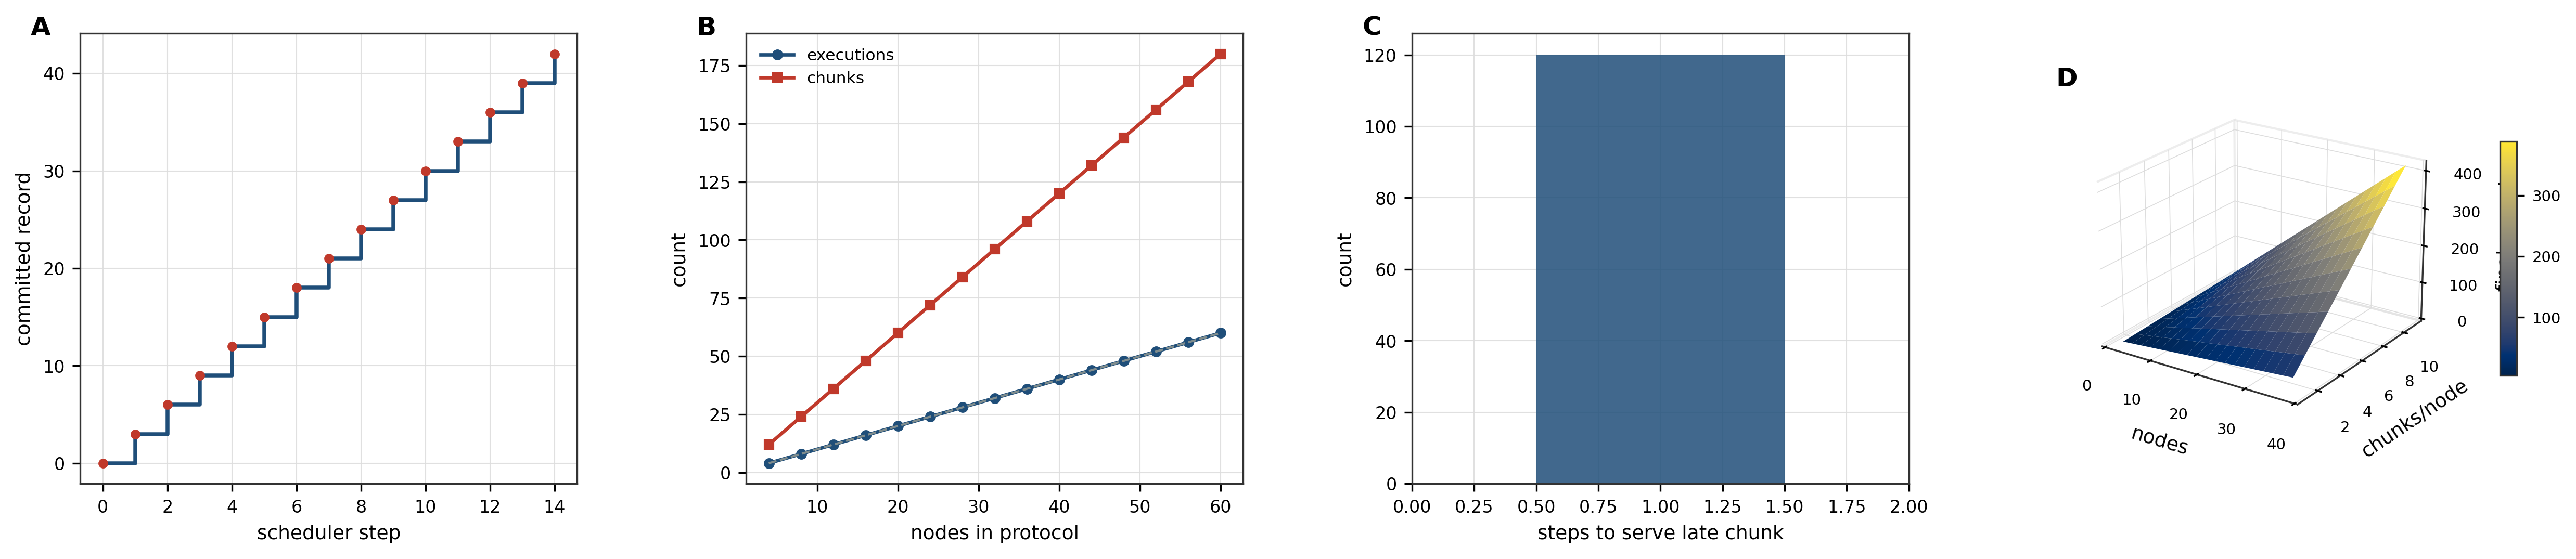
\includegraphics[width=\textwidth]{figures/panel_4_scheduler.png}
    \caption{\textbf{The committed record orders a run without a clock, and the scheduler is exact rather than merely adequate.}
    The scheduler selects uniformly at random from the ready set, which is a fair rule in the sense of \Cref{def:scheduler} but the least favourable such rule for the guarantees below; the counts are therefore not artefacts of a helpful selection order.
    (\textbf{A})~Committed record against scheduler step for a sweep over fourteen nodes carrying three chunks each. The record is a strictly increasing staircase, advancing by exactly three at each node visit and never decreasing. Because no operation in the vocabulary removes a value or decrements the count, two states with equal value stores and unequal records are distinct (\Cref{thm:monotone}): a recurring configuration is not a return, and the ordering is available without reference to wall-clock time (\Cref{cor:clock}).
    (\textbf{B})~Executions and committed chunks against protocol size. The execution count equals the node count exactly at every size tested, up to $60$ nodes, and the committed record equals the total chunk count, reaching $180$ at the largest protocol. Each node is therefore visited once and all its pending chunks are evaluated in that visit, which is the no-redundant-re-execution clause of \Cref{thm:scheduler}(i) measured rather than assumed.
    (\textbf{C})~Steps required to serve a chunk contributed \emph{after} a sweep has completed and every node has gone quiescent, over $120$ trials. Every late chunk was served in exactly one step and none was starved. The result is stronger than \Cref{thm:scheduler}(ii) requires---the theorem guarantees only eventual service---and it holds because a contribution makes its node ready again immediately, so the readiness rule needs no notion of priority or ageing.
    (\textbf{D})~Final committed record over protocol size and chunks per node. The surface is exactly the product of its two arguments, with no deviation at any grid point, confirming that the record counts committed evaluations and nothing else: no retries, no speculative execution, no bookkeeping steps enter it. This is what makes the record usable as a provenance ordinal.}
    \label{fig:kpanel4}
\end{figure*}


\subsection{Results}
\label{sec:results}

All seven checks passed. We report the quantities rather than the verdicts,
since the verdicts are uninformative on their own.

\emph{Inertia.} A node carrying five chunks, two of which raise, emitted
five values: three ordinary and two error values. The committed record
advanced to $5$, showing that a raising chunk commits exactly as a
non-raising one does. All three non-raising chunks were evaluated despite
two of the five raising, which is the content of \Cref{cor:completion}. No
attribute of the kernel object corresponded to an exit code, status, or
return code, consistent with \Cref{thm:inertia}.

\emph{Convergence.} Three contributions over four subtask identities,
overlapping on one, were merged in all $3!=6$ orders. All six produced the
same protocol fingerprint---one distinct fingerprint across six orders. The
shared identity accumulated $4$ chunks, being the union of two contributions
of two chunks each, confirming that convergence occurred rather than the
contributions remaining disjoint. Re-submitting every contribution a second
time left the fingerprint unchanged, exhibiting idempotence.

\emph{Fingerprint discrimination.} The fingerprint was stable across
construction orders, and changed when a single chunk's content changed and
when a single subtask identity changed, as \Cref{thm:fingerprint} requires.

\emph{Emergence and opacity.} Two runs of a fixed protocol whose probe
chunk consulted a varying external source produced identical protocol
fingerprints and different trajectories, instantiating
\Cref{thm:emergence}. When the two branches were arranged to deposit the
same terminal value, the terminal stores were equal, the interior
trajectories differed, and none of the three store-determined functions
probed---cardinality, sorted representation, and a cryptographic digest of
the sorted store---separated the two runs. This is the construction of
\Cref{thm:opacity}: the interior is not recoverable from the result.

\emph{Record.} The committed record traced $0\to1\to2$ over two
single-chunk nodes. The two nodes' value collections were equal at the end
of the run---a recurrence of value configuration---while the records
differed, so the two states were distinguished by the record alone. This is
the operative content of \Cref{thm:monotone}: recurrence is not return.
Re-executing a node whose chunk bag had not changed left the record
unaltered.

\emph{Scheduler.} Over $12$ nodes carrying $3$ chunks each, a fair random
selection over the ready set performed exactly $12$ executions and committed
all $36$ chunks, after which no node was ready and the scheduler halted. No
node was executed twice, confirming \Cref{thm:scheduler}(i), and the
execution count equalling the node count shows that each node's pending
chunks were evaluated in a single visit. A chunk contributed to an
already-executed node after the sweep was subsequently evaluated, confirming
the absence of starvation.

\begin{remark}[What the emergence and opacity checks jointly establish]
\label{rem:joint}
The two checks are complementary and it is worth stating what their
conjunction shows, since neither alone would suffice. The emergence check
fixes the protocol and varies the trajectory, demonstrating that the
trajectory is not a function of the protocol. The opacity check fixes both
the protocol \emph{and} the terminal store and varies the trajectory,
demonstrating that the trajectory is not a function of the result either.
Together they place the trajectory outside the closure of the two data a
reader of a run normally possesses---what was asked, and what came back---
which is the precise sense in which \Cref{cor:repro} restricts
reproducibility claims to the protocol. A system that logged only protocol
and terminal store would therefore be unable to reconstruct its own
trajectory even in principle, which is the practical argument for logging
the read-to-emit relation explicitly, as \Cref{rem:record-limits} recommends.
\end{remark}

% =====================================================================
\section{Discussion}
\label{sec:discussion}
% =====================================================================

\subsection{What the design buys}

The kernel guarantees that an anomaly is recorded rather than raised, that
independently derived decompositions merge deterministically, that the set
of questions a run addresses is fingerprintable and stable, and that the
order of events is recoverable without a clock. It makes explicit, and
proves, the limits of what can be reproduced: the protocol, not the
trajectory.

\subsection{What it does not buy}

It does not make a research result correct. Adjudication is relocated, not
eliminated: some module must eventually decide what a value means, and the
kernel's refusal to do so places that burden on modules where it is at least
visible. It does not make a run cheap---see
\Cref{rem:inertia-cost}. It does not guarantee that contributors converge:
that depends on identity formation, which is above the kernel
(\Cref{rem:identity}). And it does not permit unrestricted self-adjudication
(\Cref{sec:selfanalysis}).

\subsection{Conclusion}

The kernel's single commitment---to execute and not to judge---is shown to
be structural rather than conventional: the state space contains no
expectation, so no computed quantity can mean ``wrong''. From that
commitment follow run-to-completion under anomaly, order-independent
convergence of independent decompositions, a fingerprintable protocol, an
emergent and opaque trajectory, a monotone record, and a sound scheduler.
The most consequential result is the separation of protocol from trajectory,
because it identifies what a reproducibility claim about exploratory
computation can and cannot mean. The most consequential limitation is the
diagonal restriction on self-adjudication, which we state rather than
circumvent.

\bibliographystyle{plainnat}
\bibliography{references}

\end{document}
